\documentclass{beamer}

\usepackage[utf8]{inputenc}
\usepackage{hyperref}

\usetheme{Berkeley}
\beamertemplatenavigationsymbolsempty
\setbeamertemplate{headline}{}
 
\title{Geo-Clustering in FoodChain-Lab}
\date{}
 
\begin{document}
\maketitle

\section{ }

\subsection{Aufgaben}
\begin{frame}
	\begin{itemize}
		\item Nutzen Sie folgenden Workflow: \url{https://github.com/SiLeBAT/BfROpenLabResources/raw/master/GitHubPages/workflows/Example_Workflow.zip}
		\item Clusters Sie alle französischen Stationen mit Hilfe des \textbf{GIS Cluster}-Knotens.
		\item Nutzen Sie dabei eine \textbf{Max Neighborhood Distance} von 100km.
		\item Das bedeutet, dass zwei Stationen in das selbe Cluster kommen, wenn Sie weniger als 100km voneinander entfernt sind.
	\end{itemize}
\end{frame}
 
\subsection{1}
\begin{frame}
	\begin{center}
  		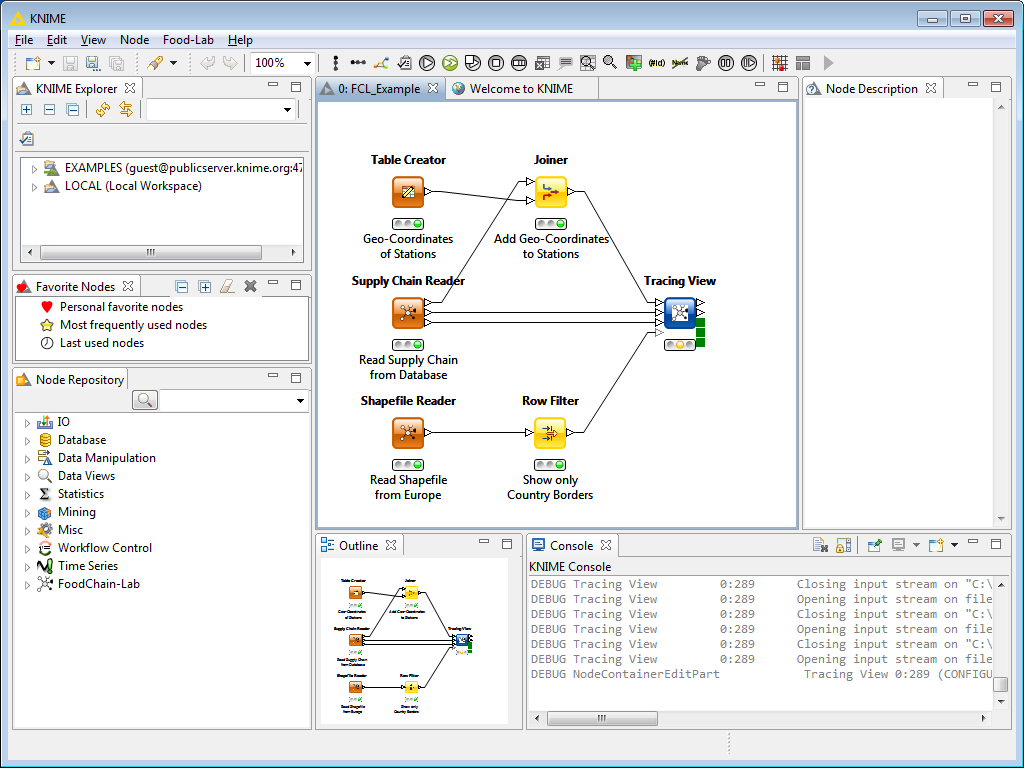
\includegraphics[height=0.6\textheight]{1.png}
	\end{center}
	\begin{itemize}
		\item Importieren Sie den Beispiel Workflow von \url{https://github.com/SiLeBAT/BfROpenLabResources/raw/master/GitHubPages/workflows/Example_Workflow.zip}.
	\end{itemize}
\end{frame}

\subsection{2}
\begin{frame}
	\begin{center}
  		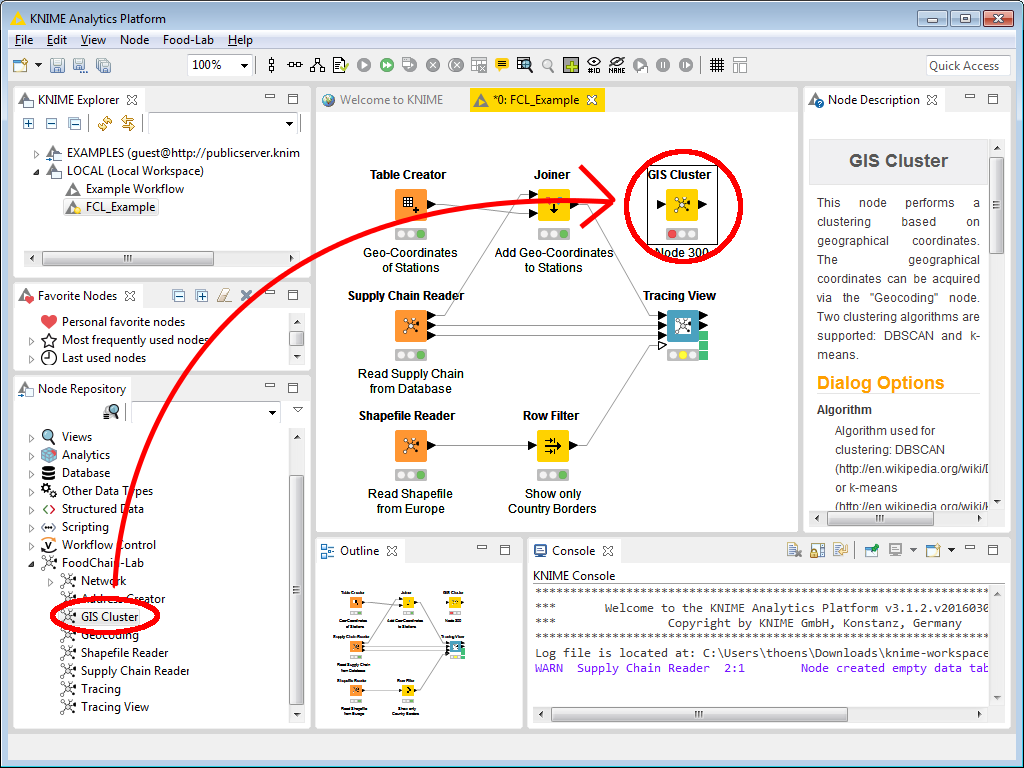
\includegraphics[height=0.6\textheight]{2.png}
	\end{center}
	\begin{itemize}
		\item Ziehen Sie den \textbf{GIS Cluster}-Knoten aus dem \textbf{Node Repository} in den Workflow.
	\end{itemize}
\end{frame}

\subsection{3}
\begin{frame}
	\begin{center}
  		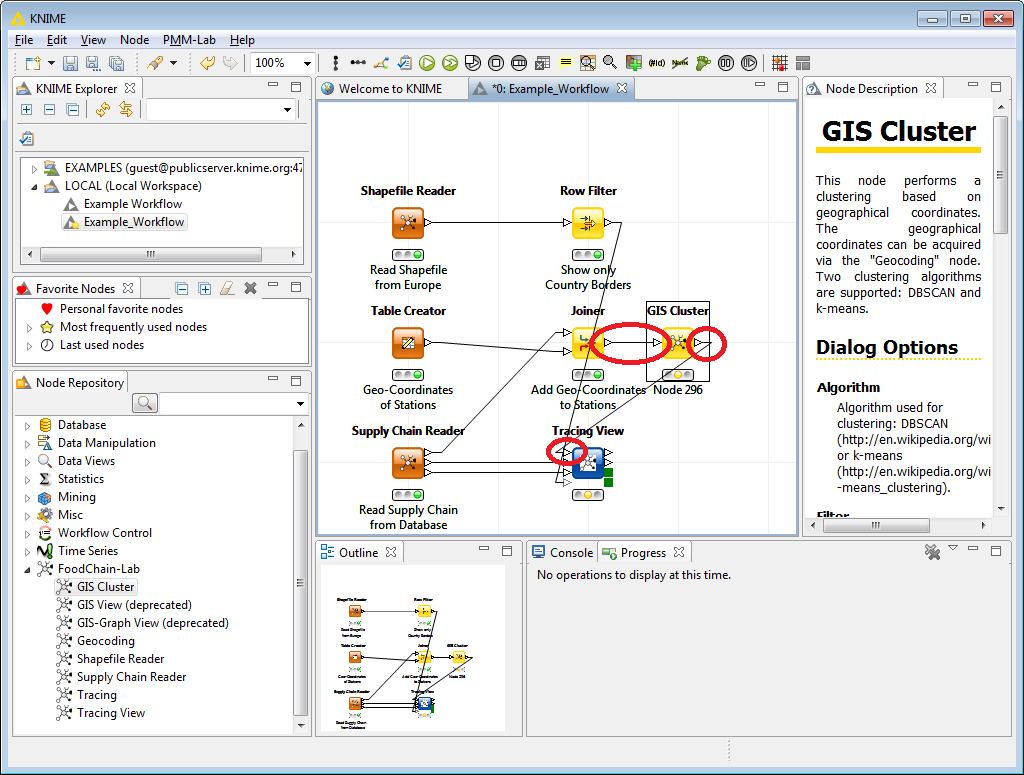
\includegraphics[height=0.6\textheight]{3.png}
	\end{center}
	\begin{itemize}
		\item Verbinden Sie den Ausgabe-Port des \textbf{Joiner}-Knotens mit dem Eingabe-Port vom \textbf{GIS Cluster}-Knoten.
		\item Verbinden Sie den Ausgabe-Port des \textbf{GIS Cluster}-Knotens mit dem Eingabe-Port vom \textbf{Tracing View}.
		\item Machen Sie einen Doppelklick auf den \textbf{GIS Cluster}-Knoten um dessen Dialog zu öffnen.
	\end{itemize}
\end{frame}

\subsection{4}
\begin{frame}
	\begin{center}
  		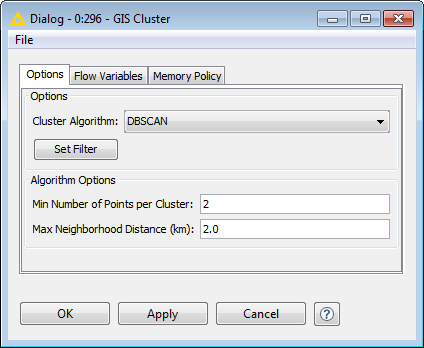
\includegraphics[height=0.6\textheight]{4.png}
	\end{center}
	\begin{itemize}
		\item In dem Dialog können den Algorithmus zum Geo-Clustern konfigurieren.
		\item Klicken Sie auf \textbf{Set Filter} um zu definieren welche Stationen geclustert werden sollen.
	\end{itemize}
\end{frame}

\subsection{5}
\begin{frame}
	\begin{center}
  		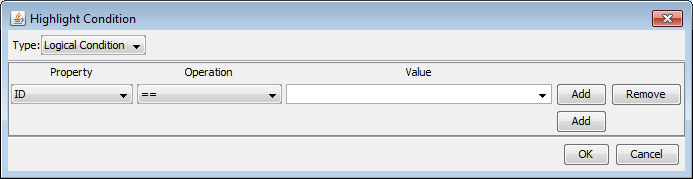
\includegraphics[width=0.9\textwidth]{5.png}
	\end{center}
	\begin{itemize}
		\item Sie sollten jetzt folgenden Dialog sehen.
	\end{itemize}
\end{frame}

\subsection{6}
\begin{frame}
	\begin{center}
  		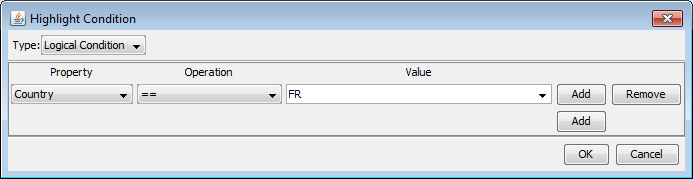
\includegraphics[width=0.9\textwidth]{6.png}
	\end{center}
	\begin{itemize}
		\item Wir wollen nur französische Stationen clustern, da sich die meisten Primärproduzenten unseres Datensatzes in Frankreich befinden.
		\item Wählen Sie "Country" als \textbf{Property} und "FR" als \textbf{Value} und klicken Sie dann \textbf{OK}.
	\end{itemize}
\end{frame}

\subsection{7}
\begin{frame}
	\begin{center}
  		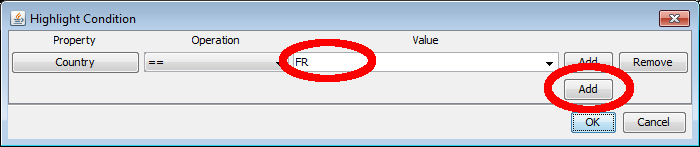
\includegraphics[height=0.6\textheight]{7.png}
	\end{center}
	\begin{itemize}
		\item Setzen Sie die \textbf{Max Neighborhood Distance} auf 100km. Stationen mit einer Distanz von unter 100km landen also im selben Cluster.
		\item Klicken Sie \textbf{OK}.
	\end{itemize}
\end{frame}

\subsection{8}
\begin{frame}
	\begin{center}
  		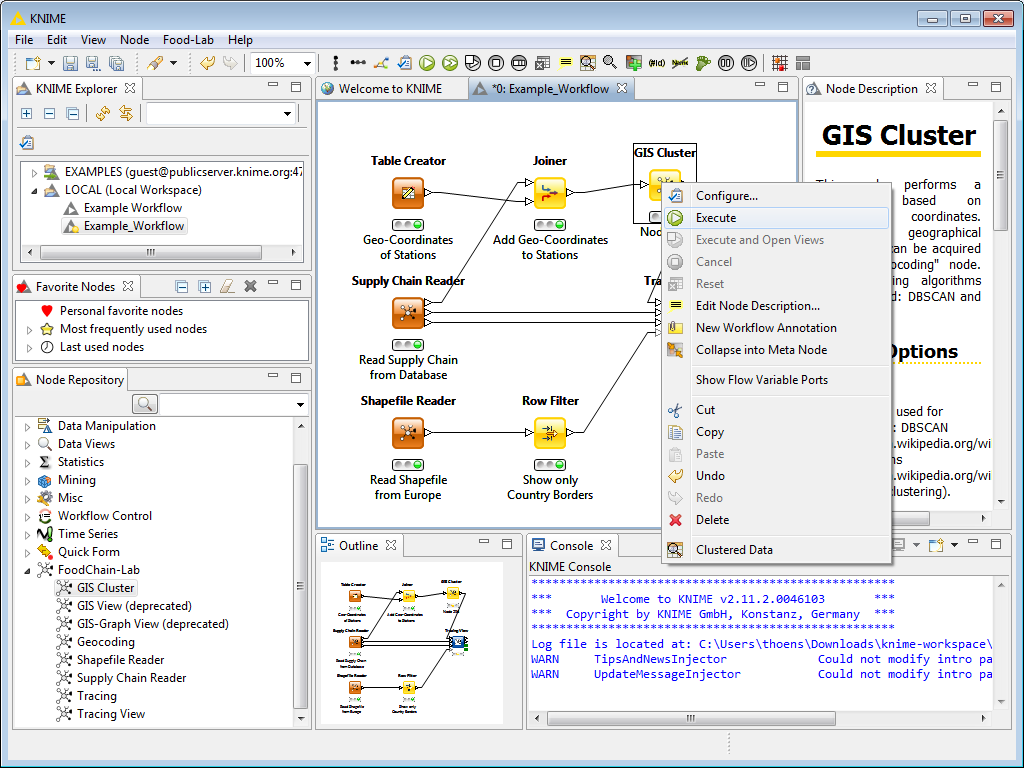
\includegraphics[height=0.6\textheight]{8.png}
	\end{center}
	\begin{itemize}
		\item Machen Sie einen Rechtsklick auf den \textbf{GIS Cluster}-Knoten und wählen Sie \textbf{Execute} um den Knoten auszuführen.
		\item Die Ergebnisse des Cluster-Algorithmus werden in der \textbf{ClusterID} Spalte gespeichert. Diese Spalte benutzen wir dann im \textbf{Tracing View}.
	\end{itemize}
\end{frame}

\subsection{9}
\begin{frame}
	\begin{center}
  		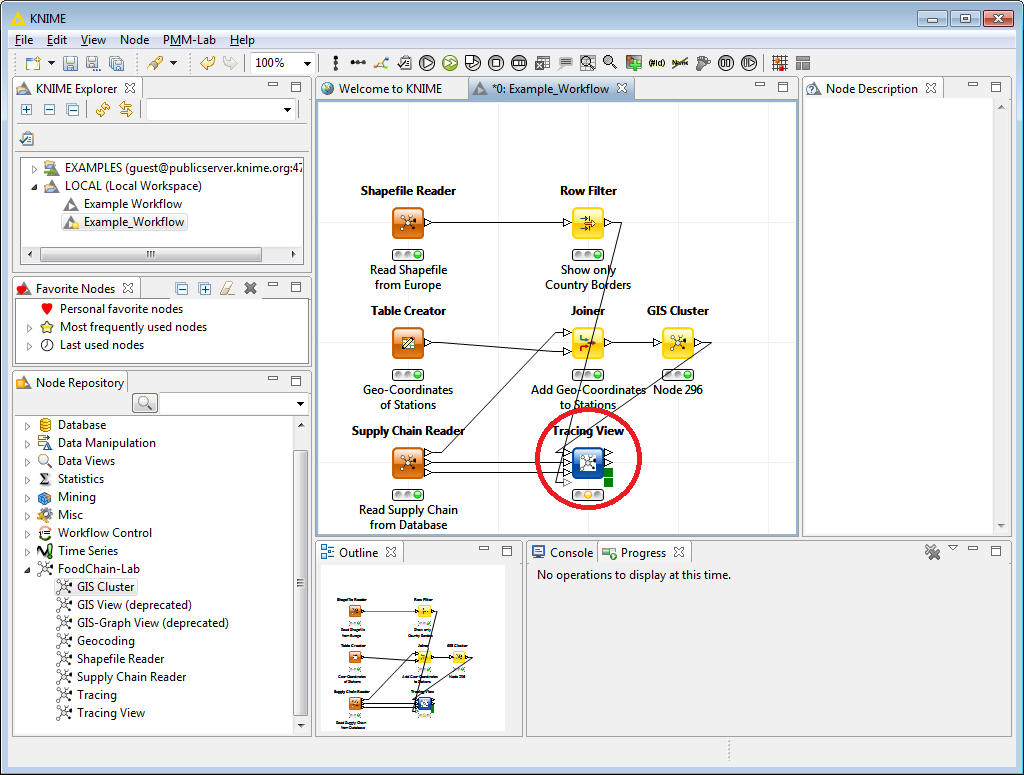
\includegraphics[height=0.6\textheight]{9.png}
	\end{center}
	\begin{itemize}
		\item Öffnen Sie den \textbf{Tracing View} per Doppelklick.
	\end{itemize}
\end{frame}

\subsection{10}
\begin{frame}
	\begin{center}
  		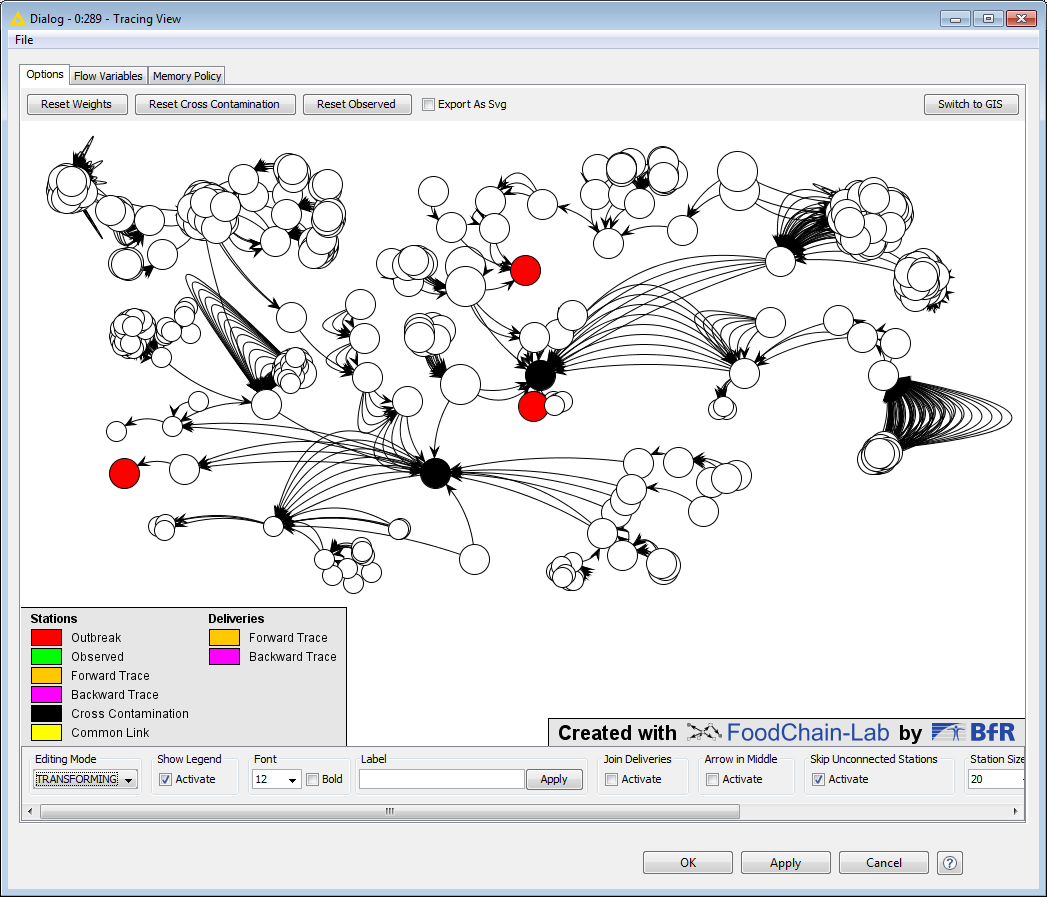
\includegraphics[height=0.6\textheight]{10.png}
	\end{center}
	\begin{itemize}
		\item Sie sollten nun ein Fenster mit dem Liefernetz-Graphen sehen.
	\end{itemize}
\end{frame}

\subsection{11}
\begin{frame}
	\begin{center}
  		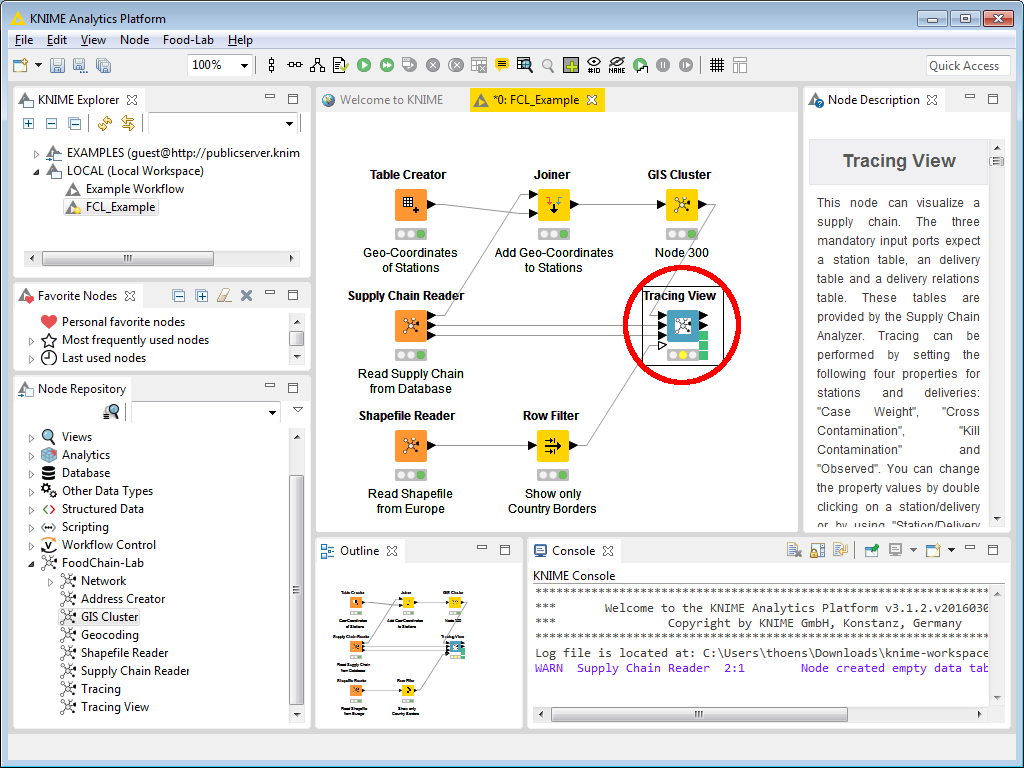
\includegraphics[height=0.6\textheight]{11.png}
	\end{center}
	\begin{itemize}
		\item Machen Sie einen Rechtsklick in den Graphen und wählen Sie \textbf{Collapse by Property}.
	\end{itemize}
\end{frame}

\subsection{12}
\begin{frame}
	\begin{center}
  		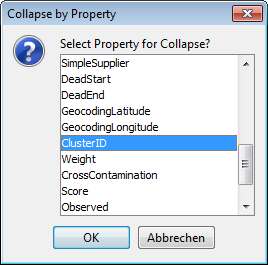
\includegraphics[height=0.5\textheight]{12.png}
	\end{center}
	\begin{itemize}
		\item Hier benutzen wir die \textbf{ClusterID}-Spalte mit den Ergebnissen vom \textbf{GIS Cluster}-Knoten.
		\item Wählen Sie \textbf{ClusterID} und klicken Sie \textbf{OK}.
	\end{itemize}
\end{frame}

\subsection{13}
\begin{frame}
	\begin{center}
  		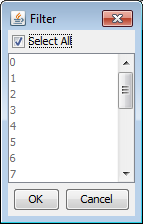
\includegraphics[height=0.5\textheight]{13.png}
	\end{center}
	\begin{itemize}
		\item Klicken Sie einfach auf \textbf{OK}, da wir kein Cluster ausschließen wollen.
	\end{itemize}
\end{frame}

\subsection{14}
\begin{frame}
	\begin{center}
  		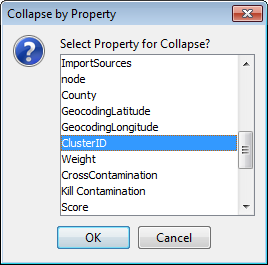
\includegraphics[height=0.6\textheight]{14.png}
	\end{center}
	\begin{itemize}
		\item Alle französischen Stationen wurden nun zu Gebieten geclustert.
		\item Jede selektierte Meta-Station (blue circle) ist ein Gebiet in Frankreich.		
	\end{itemize}
\end{frame}

\subsection{15}
\begin{frame}
	\begin{center}
  		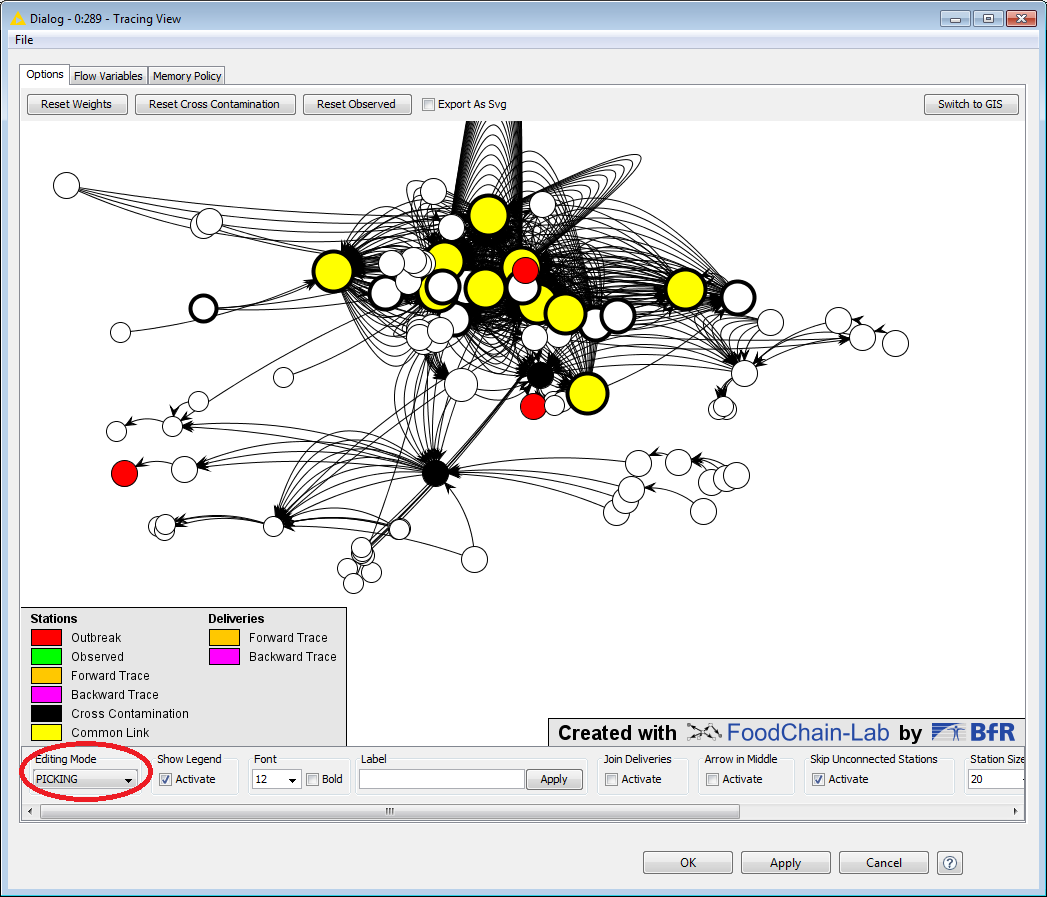
\includegraphics[height=0.6\textheight]{15.png}
	\end{center}
	\begin{itemize}
		\item Wählen Sie "PICKING" als \textbf{Editing Mode} and klicken Sie an eine leere Stelle des Graphen um alle Station zu deselektieren.
		\item Nun können Sie sehen, dass einige der Meta-Station gelb sind. Das bedeutet, dass diese französischen Gebiete eine Verbindung zu allen Ausbruchs-Stationen haben.
	\end{itemize}
\end{frame}

\subsection{16}
\begin{frame}
	\begin{center}
  		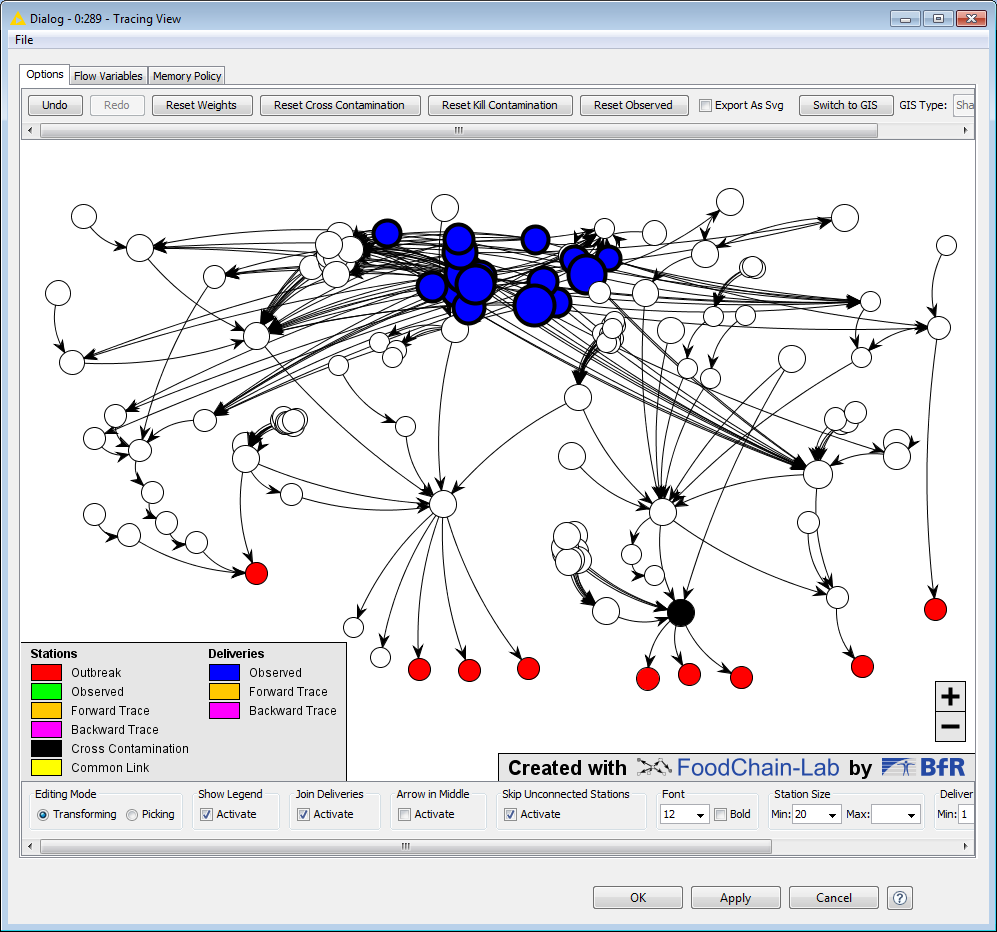
\includegraphics[height=0.6\textheight]{16.png}
	\end{center}
	\begin{itemize}
		\item Da der Graph jetzt recht unübersichtlich aussieht, sollten einen Layout-Algorithmus anwenden.
		\item Machen Sie einen Rechtsklick in den Graphen und wählen Sie \textbf{Apply Layout $>$ Fruchterman-Reingold}.
	\end{itemize}
\end{frame}

\subsection{17}
\begin{frame}
	\begin{center}
  		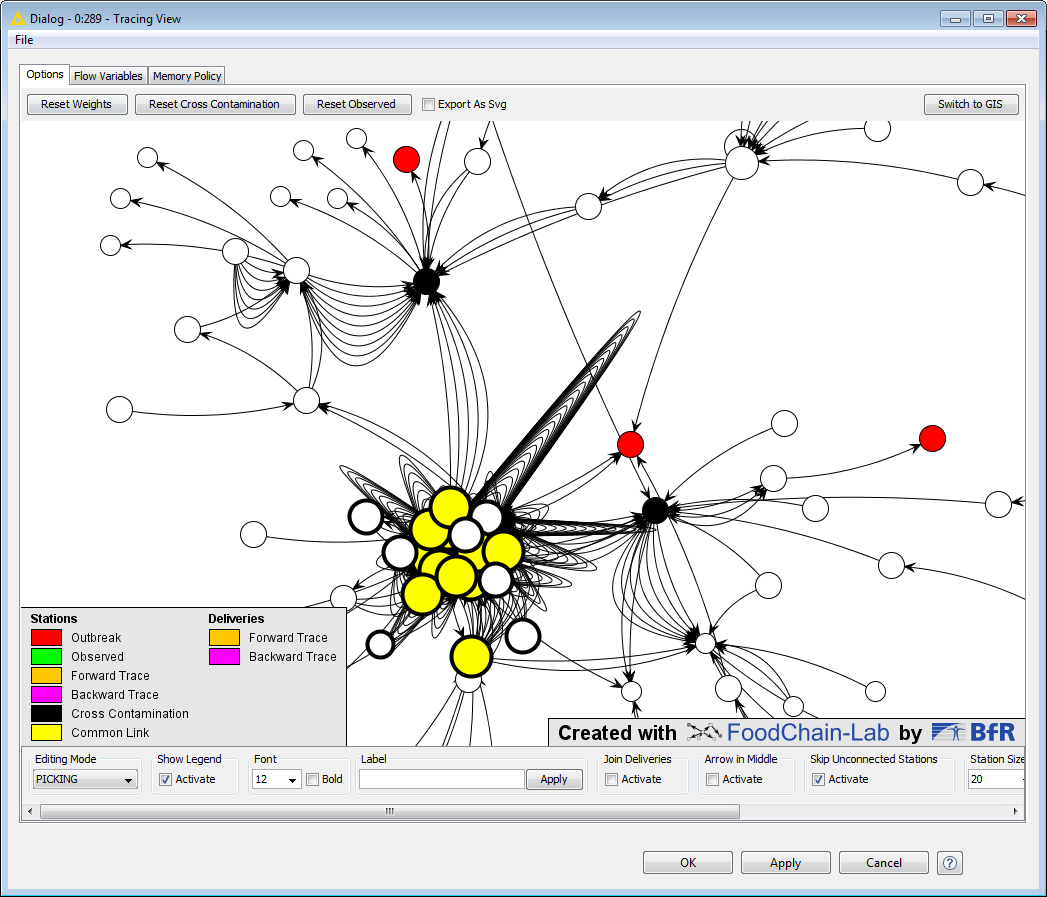
\includegraphics[height=0.6\textheight]{17.png}
	\end{center}
	\begin{itemize}
		\item Der Graph sollte jetzt übersichtlicher angeordnet sein.
		\item Der Algorithmus ist nicht deterministisch. Deshalb wird ihr Graph anders aussehen als der Screenshot hier.
	\end{itemize}
\end{frame}

\subsection{18}
\begin{frame}
	\begin{center}
  		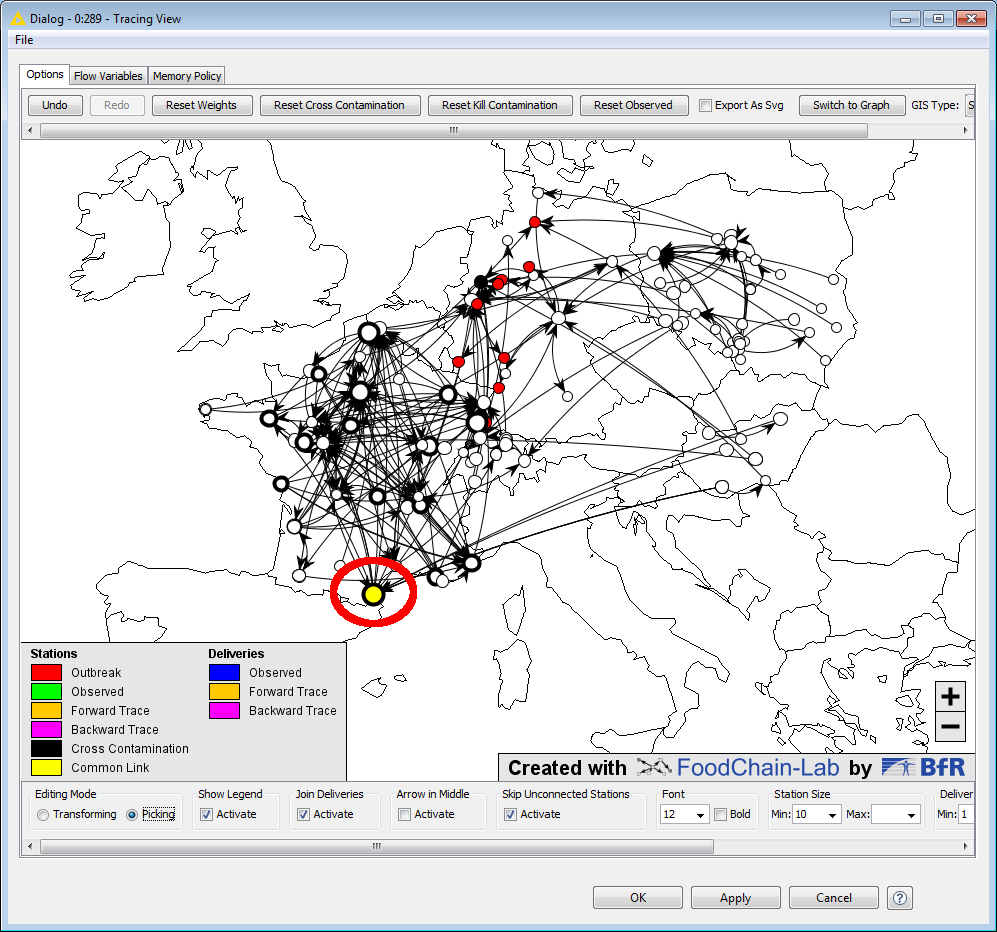
\includegraphics[height=0.6\textheight]{18.png}
	\end{center}
	\begin{itemize}
		\item Nach Anwenden des Layout-Algorithmus sind einige Stationen nicht mehr im sichtbaren Bereich.
		\item Um den ganzen Graphen zu sehen, wählen Sie "TRANSFORMING" als \textbf{Editing Mode} and zoomen Sie bis Sie den ganzen Graph sehen können (Zoomen funktioniert wie in Google Maps).
	\end{itemize}
\end{frame}

\end{document}